\setcounter{figure}{0}

\section{20th November 2023: Minister in the marketplace}
\subsection*{Text: Ephesians 4:11-12}
  \begin{quote}
    [11] And he gave the apostles, the prophets, the evangelists, the shepherds and teachers, [12] to equip the saints for the work of ministry, for building up the body of Christ,
  \end{quote}
\subsection*{Notes}
\begin{itemize}
  \item{Good resource: \url{www.theologyofwork.org}}
  \item{Today is mission sunday, so is next week. Some of us, when we think
  of missions, think that it doesnt concern us since we arent missionaries.
  That is not true. The primary mission of the church is to make disciples,
  not just converts. The church gives us resources and trains us to be
  disciple makers, so we can go forth to make disciples of all nations
  (Jesus’ great commission)}
  \item{For most of us, there is a gap between our sundays, and our
  monday-saturday. And most of the time in the week we spend it at the
  workplace. So the ratio is like 2 hrs to 166 hours lol. So if for us God is
  not at our workplace, then we will be living 166 hours without God :(. So we need to have the correct view of God’s role in our work!}
  \item{Three Vs for today:}
  \item{First point: vocation or occupation? As per our text, the
  pastors/etcs are given to us to train us to be godly people. Vocation:
  vocation for the christian is a matter of responding to God’s call on all
  believers to be faithful. Occupation is a career that we select to earn a
  living.}
  \item{To be a pastor etc, is just one’s occupation, much like being an
  engineer. Being a pastor is not “holier” than being an engineer. But those
  are just occupations, the vocation for both is the same; to be faithful
  christians! The goal is to make it such that our occupation aligns with our
  vocation, regardless of whether our occupation is church work or not. E.g,
  Joseph was a great administrator in Egypt, he wasnt a preacher or a pastor,
  yet he was faithful and served God. Similarly, Daniel. }
  \item{So for most of us, our occupation is at the marketplace. On sunday we
  come to be trained by the pastors, on mon-sat we are the “pastors” to the
  world! God is working not just on sunday, but on mon-sat, through us to the
  world at the marketplace!
  \begin{itemize}
    \item{On Sunday, we ``come to church'', on Mon-Sat, we ``be the
    church''.}
    \item{On Sunday, it is ``I go to church'', on Mon-Sat, it is ``I am the
    church''.}
    \item{On Sunday, it is about ``belonging'' (becoming a child
  of God), on Mon-Sat, it is about ``being'' (Sharing Christ,
  Chirst-likeness).}
  \end{itemize}}
  \item{We must not be christians who are one way on sunday, and another way on mon-sat. We must make our occupation align with our vocation!}
  \item{The church exists, called out of the world, not to escape the world, but to be cleansed, nourished, and then sent out to be a light to the world.}
  \item{Vision or work: from our text, we see that the church is the equipping centre, the marketplace is the mission field. }
  \item{Our text is misunderstood when we read it to mean that the pastors
  are doing two jobs; equipping the saints and doing the work of ministry.
  But actually, the proper understanding is as per shown in the ESV; the
  pastors just have one job (to equip the saints for the work of ministry)
  and the rest of us have the other job, to do the work of ministry.}
  \item{Re-thinking pastors: Pastors are not called to get people to assist them in their ministry. Rather, the pastor is called to assist the people, the ``laity'', with their ministry both in the church and in the world.}
  \item{Questions: how can we make our occupation a platform to share about Jesus?}
  \item{We need to relook at our vocation, to see how we can use it to share
  our faith. Some general rules are:
  \begin{itemize}
    \item{Just spend more time at the workplace making casual conversations
    with people, walk through the pantry when you go to the toilet, eat lunch
    with people, etc etc. If better, try to see if you can create a
    hospitable culture where people feel free to share about their personal
    life, then you can also share about your personal life :).}
  \end{itemize}
  A more specific example is, if you are a businessman, try to see if you can
  do business as a means for missions! This is usually the way, especially in
  “creative access countries”. }
  \item{When Christians think about “serving God”, they often think about the “equipping” portion, like being a DGL, serving in the choir, etc. While serving God is more than that, (as mentioned, we also serve God in the marketplace), equipping the rest of the saints is also important! This is why those who serve in church have to think about the importance of their role.}
  \item{“The church does not exist to entertain the saved. It exists to train disciples to glorify God and to reach the lost.
  \begin{figure}
    \centering
    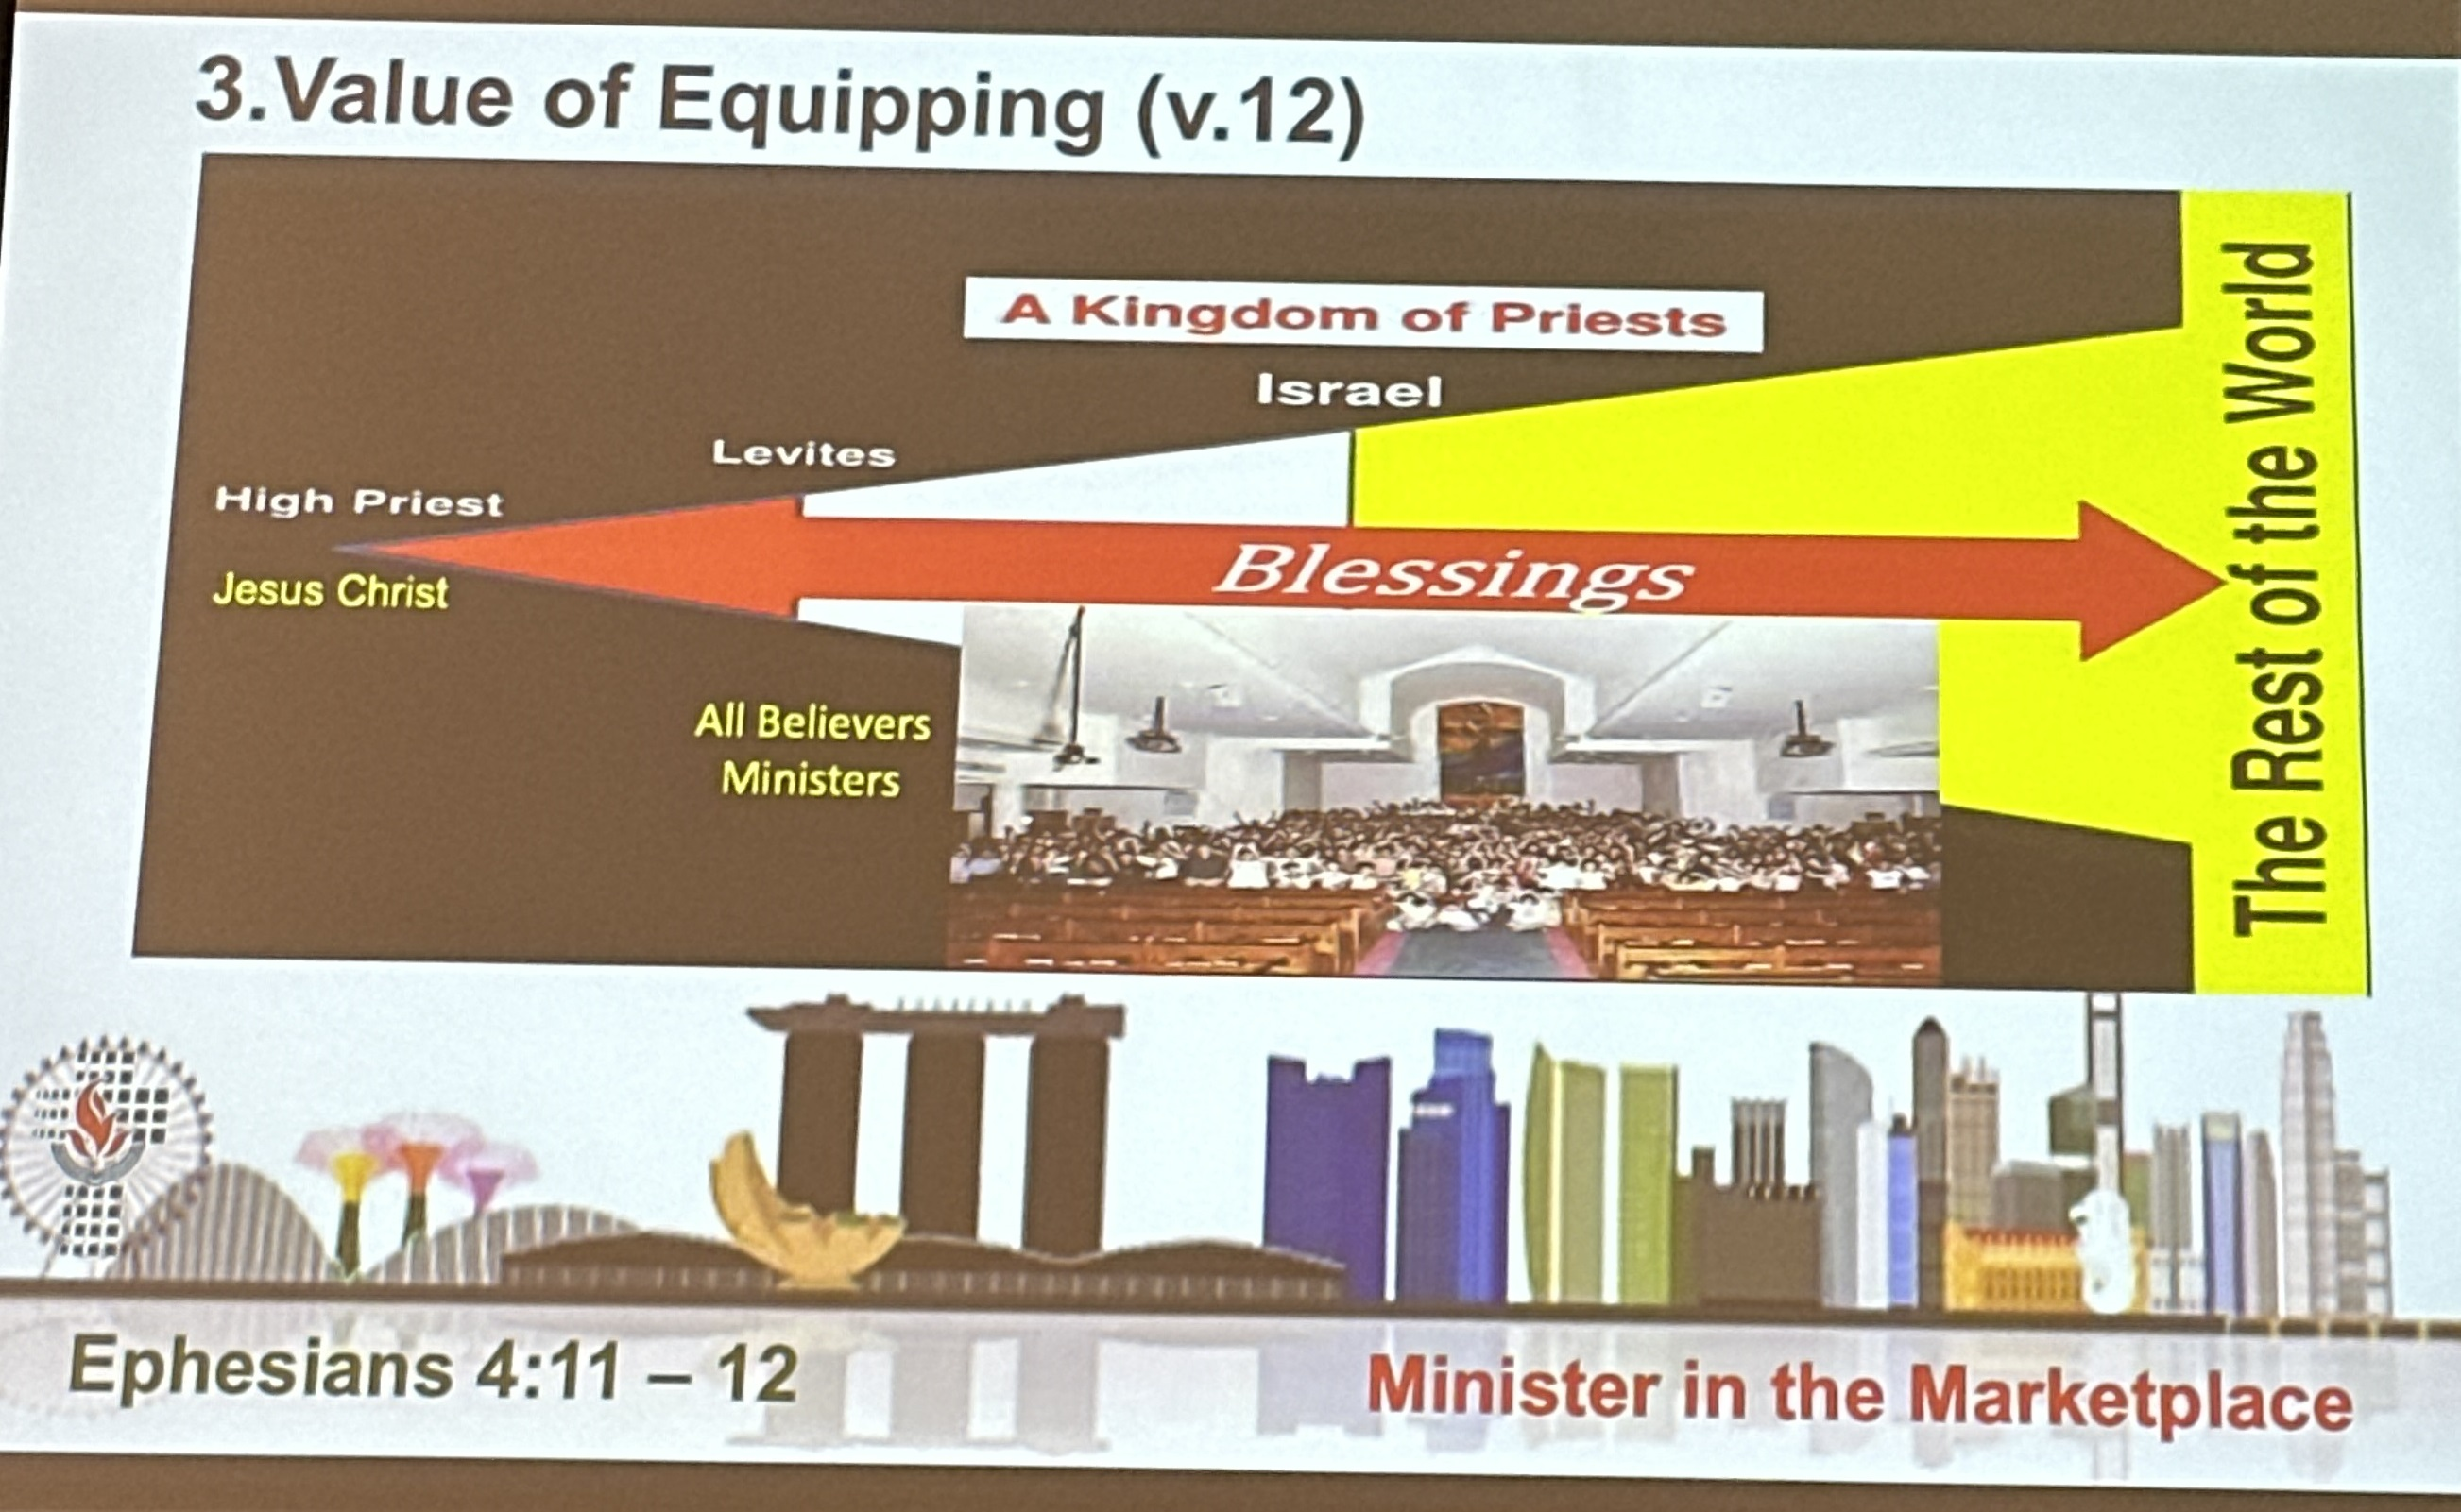
\includegraphics[width=0.8\textwidth, trim={0cm 0cm 0cm 0cm},clip]{Figures/novemberSermon3Fig1.jpg}
    \caption[]{}
    % \label{}
  \end{figure}
  }
  \item{For Mon-sat, the local church exists in scattered form, and we share about Jesus through our own relationships with the people around us at work, and if possible, by using our work as a platform.}
  \item{Applications for us:
  \begin{enumerate}
    \item{As a working Christian, have you prayed for the salvation of your colleagues, employees, and superiors who do not yet believe in the Lord?}
    \item{Do you approach your workplace with a sense of mission? Or do you, like those who do not believe, approach the workplace with an "it's not my concern" attitude?}
  \end{enumerate}
  \item{Quote from Mark Greene: The workplace is incredibly strategic for
  mission and ministry. We spend 50 to 70\% of our waking hours there. 'It's
  the one place where Christian and non-Christian have to meet. The one place
  where the playing field is even, where Christian and non-Christian are
  subject to the same corporate culture, the same pressures. The one place
  where the non-Christian can actually see the difference that Christ can
  make to a life - not for a couple of hours over dinner but for 20, 30, 40,
  50 hours a week over a couple of years.... Often the people who know us
  well don't live next door, they work at the next desk.' Note how many TV
  shows are set in the workplace - police, law firms, hospitals. That's where
  the drama and life-changing decisions take place.}
  }
  % \item{\begin{figure}[H]
  %   \centering
  %   % 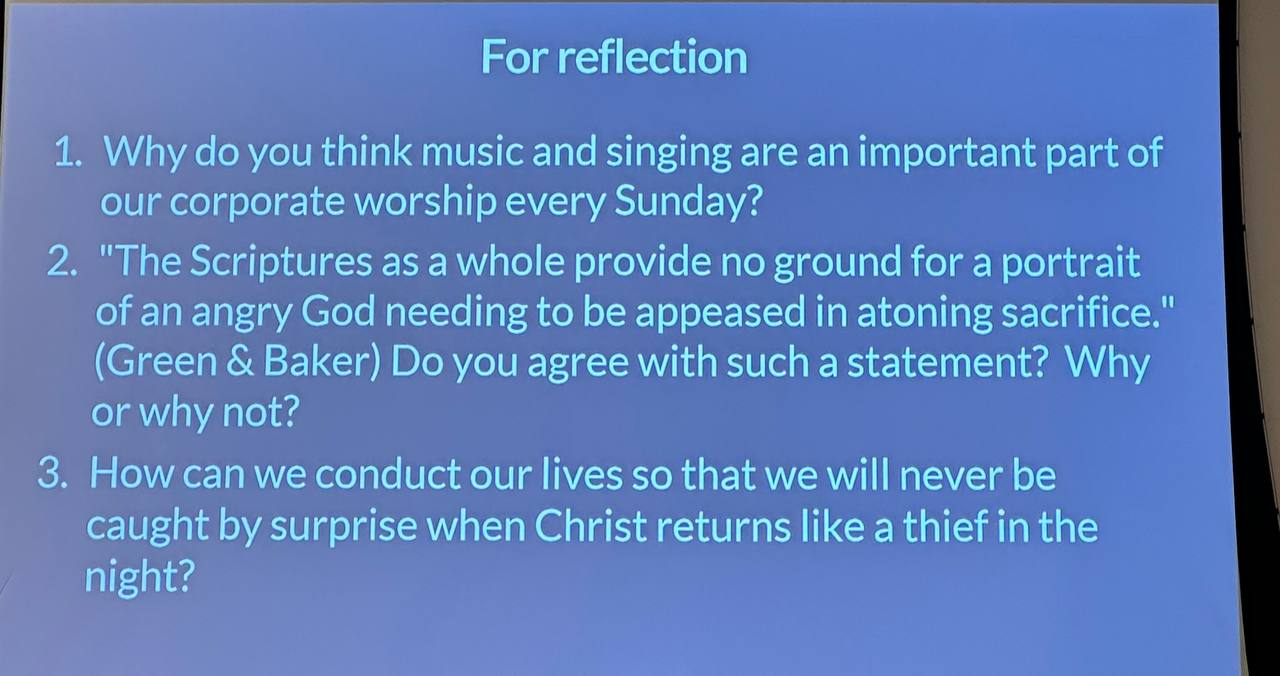
\includegraphics[width=0.8\textwidth, trim={0cm 0cm 0cm 0cm},clip]{Figures/marchSermon4Reflections.jpg}
  %   \includegraphics[width=0.8\textwidth, trim={0cm 0cm 0cm 0cm},clip]{example-image-a}
  %   \caption[]{Reflection questions for this sermon}
  %   \label{}
  % \end{figure}}
\end{itemize}